\subsubsection{Study concurrent use of resources at architectural level (PT Net)}\label{subsubsection: study concurrent use of resources at architectural level (PT Net)}

It is necessary to model distributed systems to study the concurrent use of resources at the architectural level.

\highspace
A \definition{Petri Net (PT Net or P/T Net)}, a place/transition net (PT net), is one of several \textbf{mathematical modelling languages used to describe distributed systems}. Like industry standards such as UML activity diagrams, \textbf{Petri nets offer a graphical notation for stepwise processes} that include choice, iteration, and concurrent execution.

\highspace
The Petri net uses a graphic tool. It is a bipartite-directed graph containing places (circles), transitions (bars), and directed arcs.

\highspace
A Petri net is a four-tuple:
\begin{equation}
    PN = <P, T, I, O>
\end{equation}
\begin{itemize}
    \item $P$: a \textbf{finite set of places} $\left\{p_{1}, p_{2}, \dots, p_{n}\right\}$
    
    \item $T$: a \textbf{finite set of transitions} $\left\{t_{1}, t_{2}, \dots, t_{s}\right\}$
    
    \item $I$: an \textbf{input function} $\left(T \times P\right) \longrightarrow \left\{0,1\right\}$
    
    \item $O$: an \textbf{output function} $\left(T \times P\right) \longrightarrow \left\{0,1\right\}$
\end{itemize}
It's also possible to add another term called $M^{0}$, which is an \textbf{initial marking} $P \longrightarrow N$:
\begin{equation}
    PN = <P, T, I, O, M^{0}>
\end{equation}
Formula called also \textbf{marked Petri net}.

\highspace
You can find a detailed explanation \href{https://isr.umd.edu/Labs/CIM/miscs/wmsor97.pdf}{here}. Some observations of the Petri net:
\begin{itemize}
    \item In a given marking $M$, a transition $t$ can fire only if it is enabled.

    \item An enabled transition not necessarily fires.

    \item More than one transition can be enabled in a marking.

    \item If two transitions are enabled at the same time:
    \begin{itemize}
        \item Which one fires first is not determined;
        \item Petri nets are an intrinsically nondeterministic model;
        \item The firing of a transition might disabled another enabled transition.
    \end{itemize}
\end{itemize}
In fact, if two transitions are enabled at the same time, they can fire simultaneously unless the firing of one transition disables the other. Petri nets are \textbf{suitable for modelling concurrent systems}. On \href{http://petrinet.org/}{this page} you can see a live simulation by clicking on the nodes.

\newpage

\begin{figure}[!htp]
    \centering
    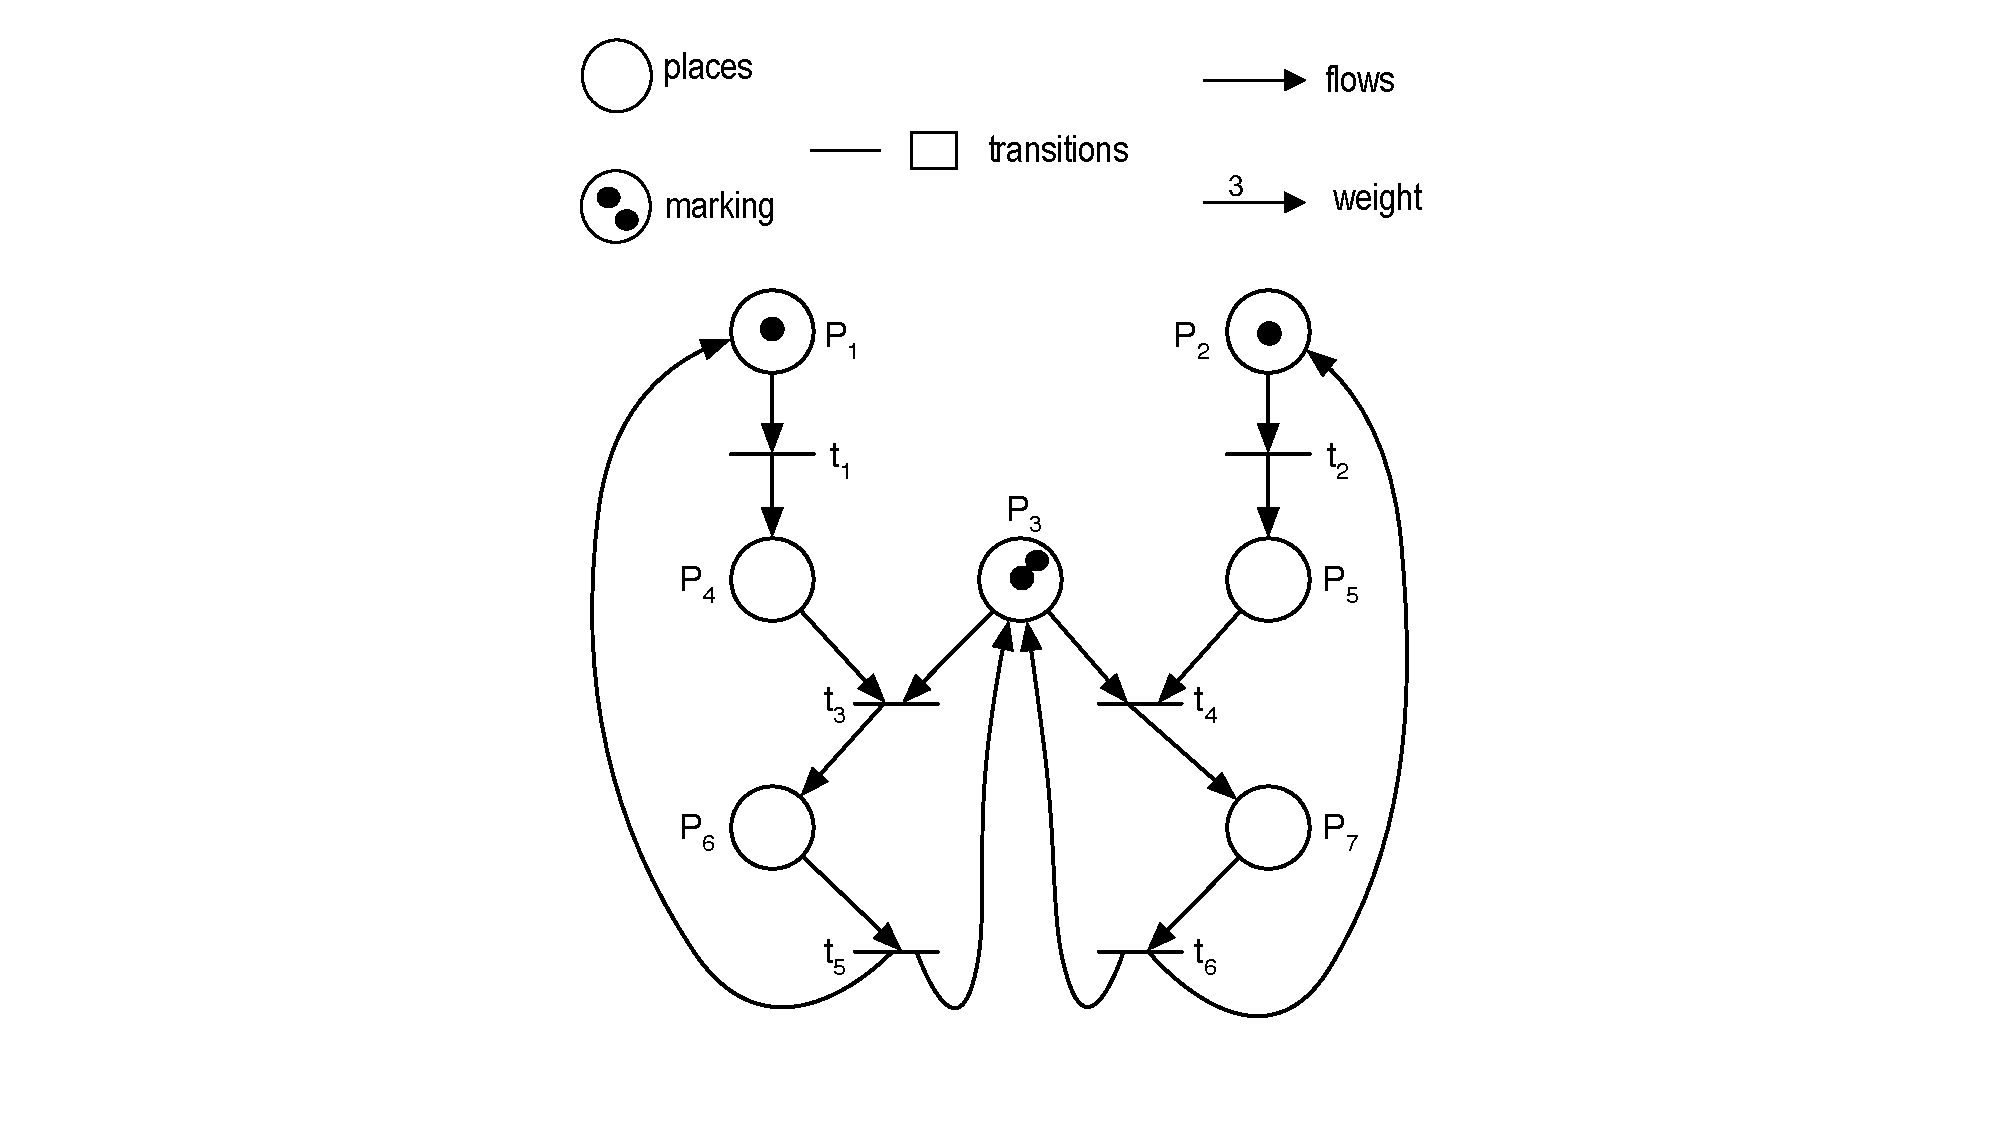
\includegraphics[width=.6\textwidth]{img/petri-nets-1.pdf}
    \caption{\example{Example} of Petri nets.}
\end{figure}

\begin{figure}[!htp]
    \centering
    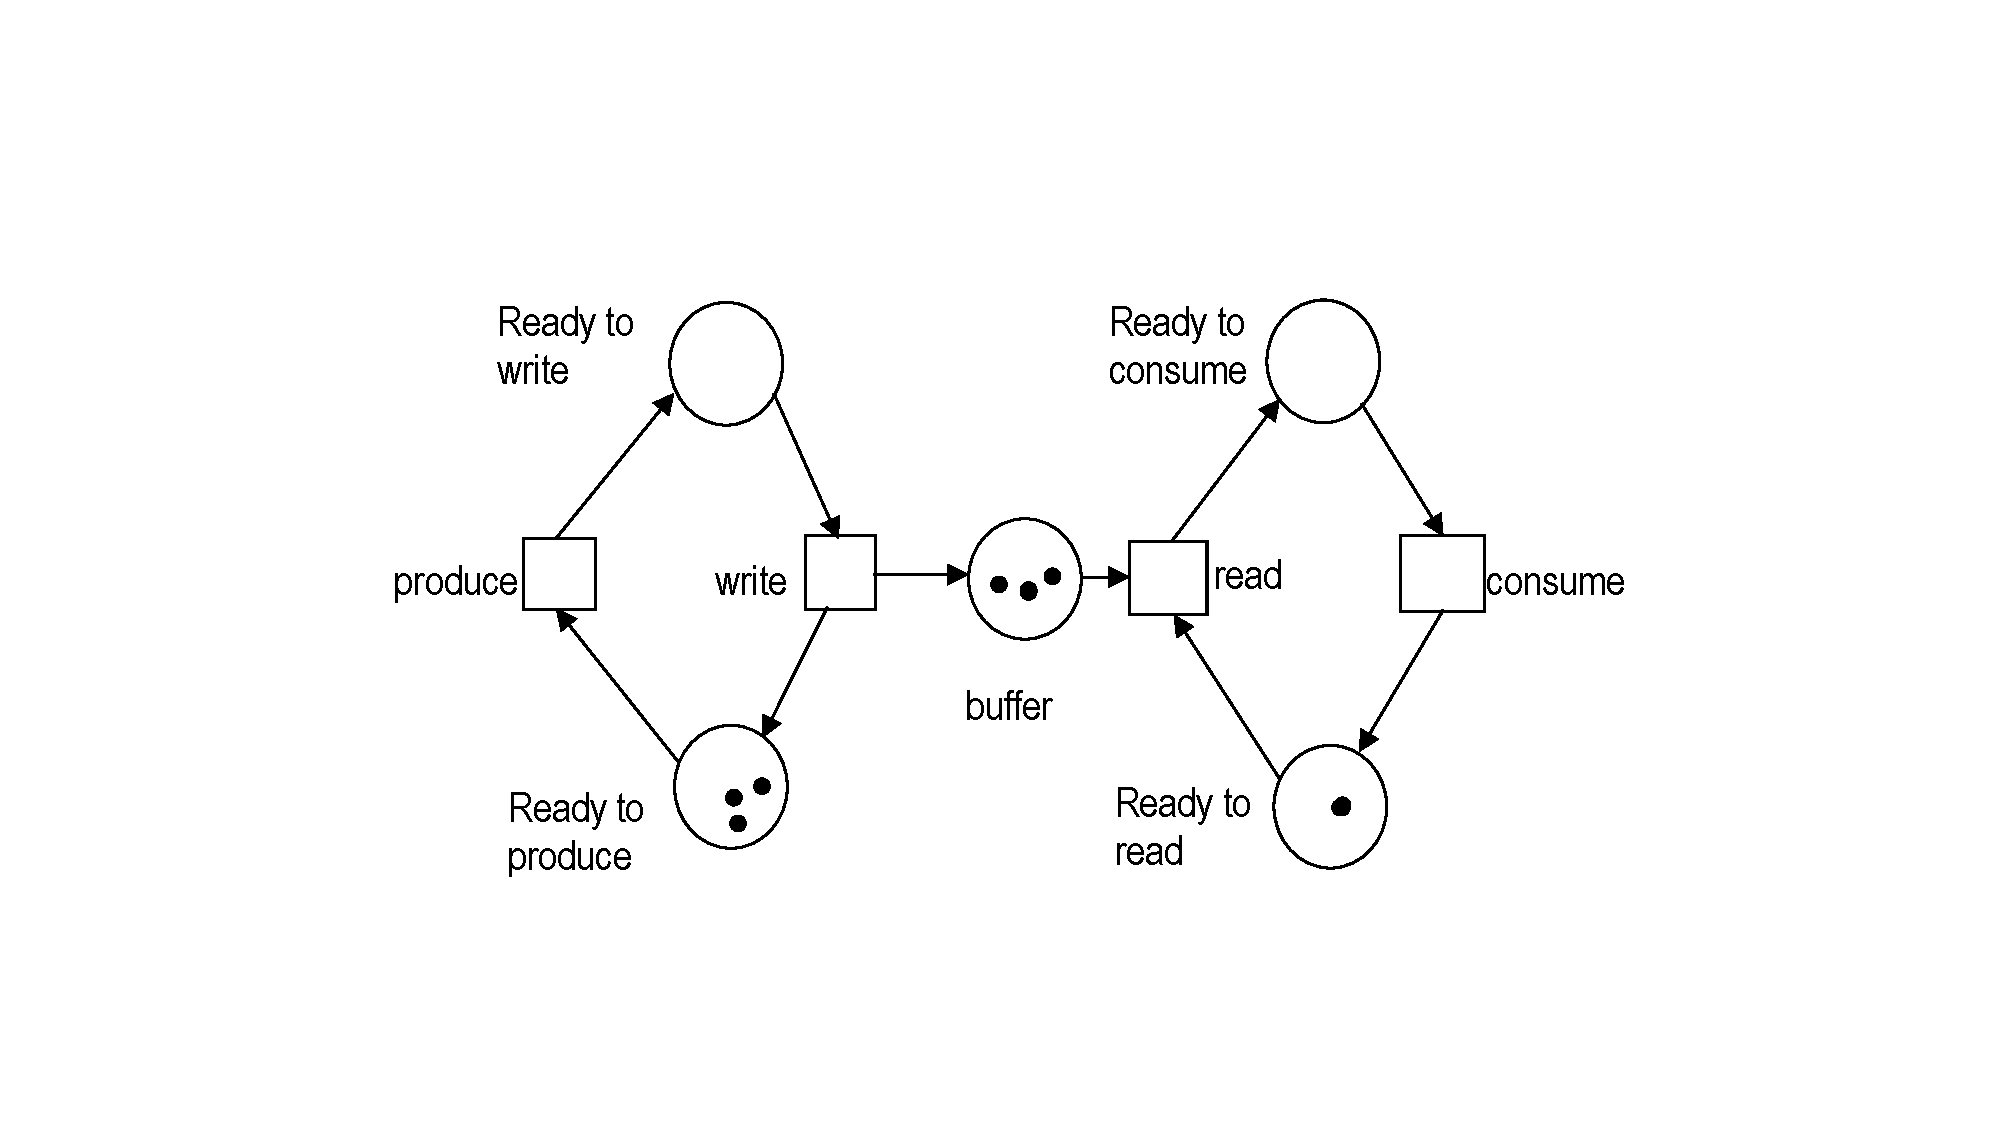
\includegraphics[width=.9\textwidth]{img/petri-nets-2.pdf}
    \caption{\example{Example} of Petri nets of producer-consumer model with unbounded buffer.}
\end{figure}

\newpage

\begin{figure}[!htp]
    \centering
    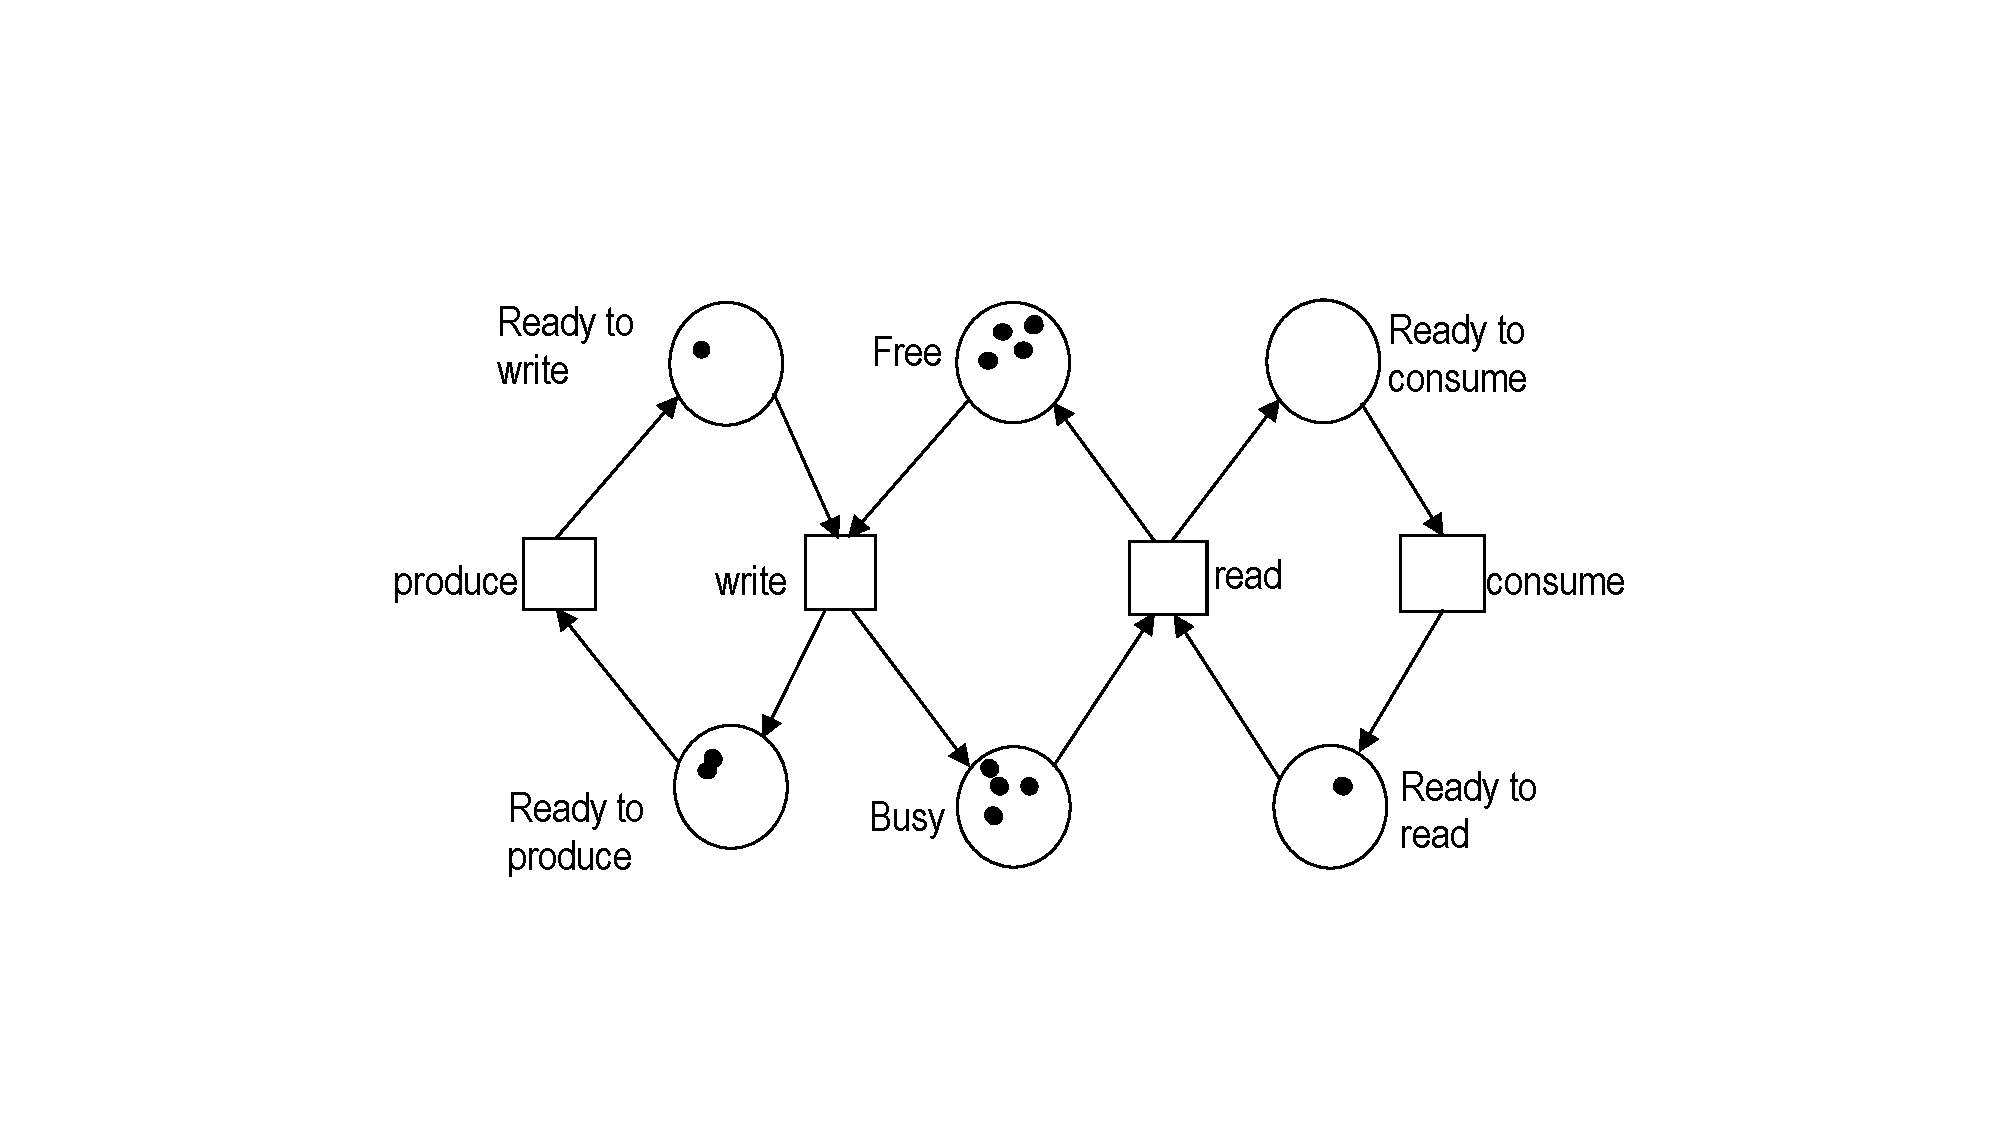
\includegraphics[width=.9\textwidth]{img/petri-nets-3.pdf}
    \caption{\example{Example} of Petri nets of producer-consumer model with finite buffer with a parametric number of positions.}
\end{figure}

\begin{figure}[!htp]
    \centering
    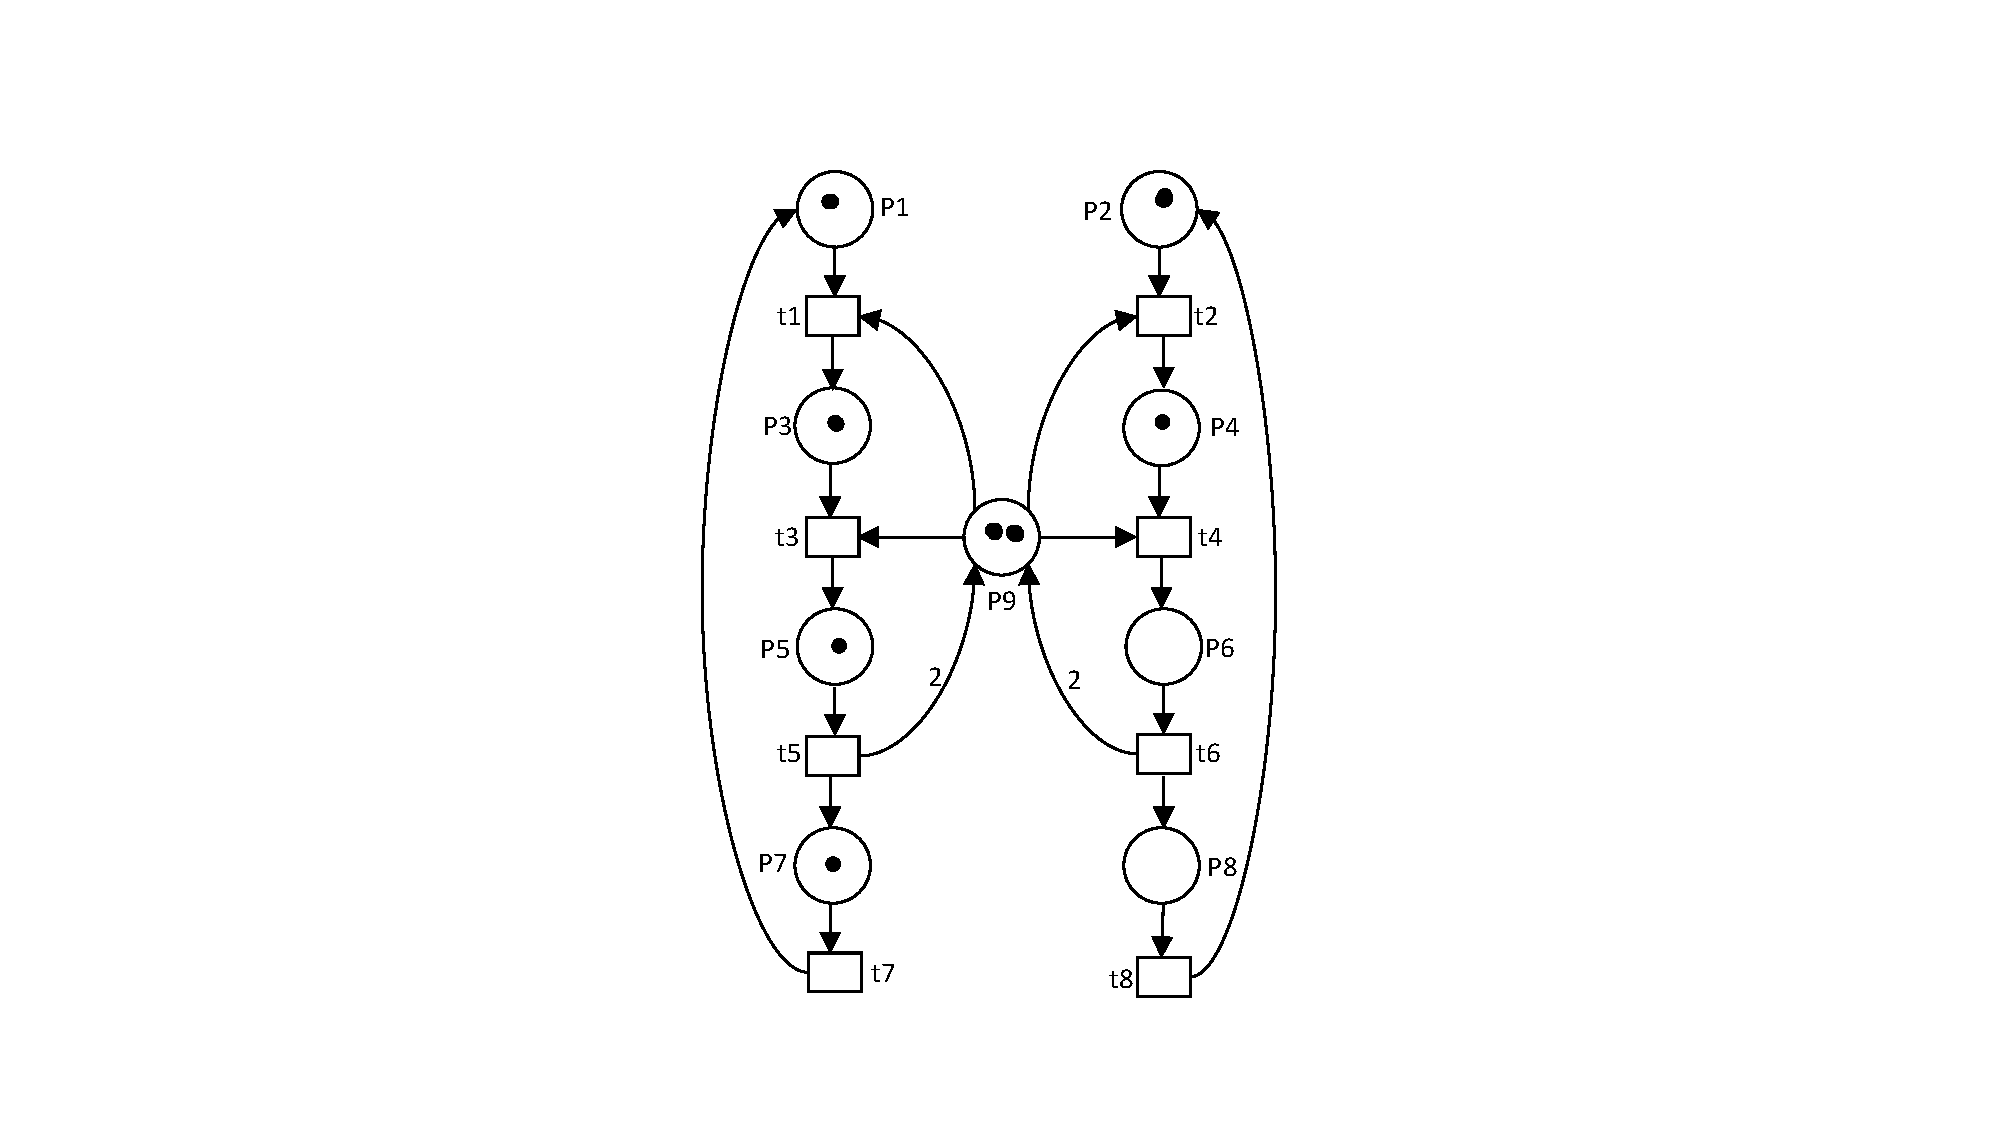
\includegraphics[width=.6\textwidth]{img/petri-nets-4.pdf}
    \caption{\example{Example} of Petri nets of deadlock.}
\end{figure}